\documentclass[a4paper]{article}

%% Language and font encodings
\usepackage[english]{babel}
\usepackage[utf8x]{inputenc}
\usepackage[T1]{fontenc}

%% Sets page size and margins
\usepackage[a4paper,top=3cm,bottom=2cm,left=3cm,right=3cm,marginparwidth=1.75cm]{geometry}

%% Useful packages
\usepackage{amsmath}
\usepackage{graphicx}
\usepackage[colorinlistoftodos]{todonotes}
\usepackage[colorlinks=true, allcolors=blue]{hyperref}

\title{Reporte de Actividad 9: Sistema de Algebra Computacional Maxima.}
\author{Jesús Antonio González Espinosa \\ \\ Física Computacional 1}
\date{Sábado, 28 de Abril del 2018}
\begin{document}
\maketitle

\section{Introducción: ¿Qué es Maxima?}

Este reporte presenta los resultados de la actividad 9 del curso: un breve manual del software Maxima. A partir de tutoriales y exploración del software se ha construido tal sumario de las características y funciones importantes de éste software. Antes de proseguir con el manual, se hablará un poco de qué es y los antecedentes de este software.

Un Sistema de Algebra Computacional es un software matemático que tiene la capacidad de manipular expresiones matemáticas de manera similar a la forma manual tradicional. Macsyma es uno de los Sistemas de Álgebra más antiguos, creado en el Instituto de Tecnología de Massachusetts (MIT). El proyecto inició en 1960, pero para 1980, el código fue llevado a varias plataformas, en donde en una de ellas se creo Maxima. Hasta la fecha, Maxima sigue siento un software libre que está en constante actualización por un grupo de desarrolladores de forma voluntaria. Existen varias interfaces para trabajar con Maxima: wxMaxima, iMaxima y xMaxima. En éste caso se va a trabajar con wxMaxima.

\section{Infraestructura de Maxima}
\subsection{Datos, Números y Variables}
En las sesiones de Maxima, cada línea tiene asociada la etiqueta $(\%i1)\%$, que significa que es la primer entrada; al escribir un comando válido terminado con un punto y coma, y presionar enter, va a aparecer el resultado con la etiqueta $(\%o1)\%$, que significa que es la primera salida. Posteriormente, va a aparecer otra etiqueta $(\%i2)\%$, y así va a seguir la sesión numerando cada entrada y salida.

Maxima acepta números reales, de forma entera, racionales o de punto flotante; también acepta números complejos. También ya se encuentran algunas constantes predefinidas, como los valores de $\pi$ (\%pi), \textit{e} (\%e), incluso \textit{i} = $\sqrt{-1}$ (\%i), donde la forma de escribirlos es lo que está entre los paréntesis. 

\bigskip

Para las variables, la forma de asociarle un valor es usando el símbolo ":", también se le puede asociar una lista de valores, al ponerlos entre corchetes y separados por una coma. Para nombrar la variable, esta tiene que ser con combinaciones de letras, números y/o los símbolos "\%", o "\_"; siempre teniendo en cuenta que Maxima es sensible a las mayúsculas y el primer carácter de la variable no puede ser un número.  

\subsection{Aritmética y Álgebra}
En Maxima, las operaciones arimeticas son a partir de los siguientes simbolos:
\begin{itemize}
\item Suma: +
\item Resta: -
\item Multiplicación: *
\item División: /
\item Exponentes: \textasciicircum
\item Raíz Cuadrada: sqrt()
\item n-esima Raíz: \^(1/n)
\end{itemize}
Con éstas, puedes hacer cálculos, como si fuera una calculadora, donde para poder evaluar, tienes que insertar un ";" al final de cada línea y dando shift + enter. 

\bigskip

Maxima siempre te va a presentar los resultados de forma exacta, a menos que le exijas que se muestre de forma decimal, con el comando "float()", donde entre paréntesis va el valor o expresión que quieres convertir a número con punto flotante. 

Para utilizar una función exponencial, se utiliza "exp()", donde entre el paréntesis va el valor al que esta elevado. Para la función logaritmo natural se utiliza "log()", donde entre paréntesis se pone el valor del logaritmo que quieres obtener. Si se quiere alguna otra base para el logaritmo, se hace mediante la formula de cambio de base.  

\bigskip

Si quieres hacer que no aparezca el valor de salida de una operación, se utiliza "\$" en vez de ";" al final de la operación. Si quieres ver el resultado de tal calculo, puedes utilizar el comando "\%;" en la próxima línea de entrada, haciendo que se imprima el último cálculo. En caso de no ser el último, solo tienes que agregar la letra "o" para hacer referencia al output, y el número de línea, entonces el comando sería así: "\%o\#;" donde \# es el número de línea donde se encuentra la operación. Puedes aplicar lo mismo si quieres rehusar esos números en futuras operaciones, solo consideras el comando como variables. 

\subsection{Funciones y Ecuaciones}

Por otra parte, Maxima también te puede mostrar operaciones matemáticas con variables algebraica, con las que pueden hacerse varias cosas a partir de comandos, dependiendo de la necesidad que haya: encontrar las raíces, simplificarla, factorizarla, expandirla, etc.

\bigskip

Para las funciones en Maxima, es muy simple, definimos la variable dependiente "f(x)", que puede ser con cualquier letra y asociarla a la función con la variable independiente mediante ":=". Para evaluar la función, en otra línea de entrada se utiliza solamente la variable dependiente "f(x)" y se sustituye x, por un valor. No hay que olvidar que al final de cada línea se tiene que poner ";".

Ahora tenemos las ecuaciones, para estas, como con una variable, tenemos que nombrarla, a partir de esto, insertamos la ecuación, en ésta sí podemos utilizar el signo "=". Por ejemplo:
\begin{center}
(\%i1) E:x\textasciicircum 2 = 4

(\%o1) $x^2 = 4$
\end{center}
En donde podemos ver que se le está definiendo el nombre E a la ecuación, y luego insertamos la ecuación. también podemos ver como se vería en la línea de entrada y la de salida. Mediante el comando "solve()" se puede solucionar una ecuación, donde se va a insertar la ecuación a resolver y luego la variable que buscamos, separados por una coma. Este es un ejemplo de un comando para las ecuaciones.

\subsection{Graficación}
Para hacer gráficas en Maxima, en este caso wxMaxima, se usa el comando "plot2d()" para gráficas en 2d, donde entre los paréntesis se van a insertar los datos de la siguiente forma:

\begin{center}
plot2d(f(x),[x,xmin,xmax])
\end{center}
Donde:
\begin{itemize}
\item f(x) va a ser la función,
\item x,xmin,xmax es el eje de la variable independiente y sus límites, respectivamente.
\end{itemize}

Para el caso de graficar en 3d, el proceso es muy parecido, ahora se utiliza el comando "plot3d()", donde entre los parentesis se van a insertar los datos de la siguiente manera:
\begin{center}
plot3d(f(x,y),[x,xmin,xmax],[y,ymin,ymax])
\end{center}
Donde:
\begin{itemize}
\item f(x,y) va a ser la función,
\item x,xmin,xmax es uno de los ejes y sus límites, respectivamente.
\item y,xmin,xmax es uno de los ejes y sus límites, respectivamente.
\end{itemize}

\bigskip
\bigskip

Esto solo es una breve introducción a la gran infraestructura de Maxima. El software cuenta con miles de comandos más para miles de necesidades, pero con lo visto hasta ahora, aporta lo necesario para poder entender el manual de integración presentado a continuación.

\section{Manual de Integración}
Maxima tiene la capacidad de hacer integrales. Se explicaran los comandos principales de integración analítica y numérica.


\subsection{Integral Indefinida}

El comando para la integral indefinida es:

\begin{center}
integrate(f(x),x)
\end{center}

donde
\begin{itemize}
\item f(x) es la función deseada a integrar.
\item x es con respecto a qué se va a integrar. 
\end{itemize}

Si solo queremos presentar como se vería la integral escrita, solo hay que poner "'" al inicio de la línea y al correrla se vera la integral, sin resolverla.

Ahora, imagina el caso en el que definas una función como una integral de otra función, valuarla no no sería permitido porque necesitamos otra variable de integración con la que queremos valuar, además de que no contamos con la constante de integración. Para resolver el problema tenemos que definir la función de la siguiente manera:

\begin{center}
f(x):= subst(t=x, integrate(g(t),t) + C;
\end{center}

En donde solucionamos el problema: estamos integrando la función con la variable t, para que después la función resultante se sustituya para que su variable independiente sea x y no t. También se encuentra considerada la constante de integración. 

\begin{figure}[h!]
  \centering
  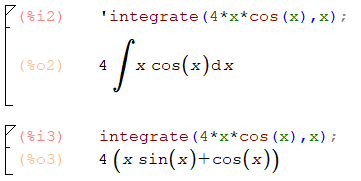
\includegraphics[width=0.4\linewidth]{indef_ej.PNG}
\end{figure}

\subsection{Integral Definida}

El comando para la integral definida es:

\begin{center}
integrate(f(x),x,a,b)
\end{center}

donde
\begin{itemize}
\item f(x) es la función deseada a integrar.
\item x es con respecto a qué se va a integrar. 
\item a es el límite inferior de integración.
\item b es el límite superior de integración.
\end{itemize}

Hay que recordar que si solo queremos presentar como se vería la integral escrita, solo hay que poner "'" al inicio de la línea y al correrla se vera la integral, sin resolverla.

\bigskip

También se cuenta con otros comandos como "defint" y "ldefinit". El primero es llamado por el comando "integrate", cuando éste se encuentra definido, y el segundo siempre se basa en los mismos métodos, por lo que es posible que no reconozca casos especiales; por ésto, es más recomendable utilizar el comando "integrate". Los comandos tienen el mismo formato el comando "integrate" para la integral definida:
\begin{center}
defint(f(x), x, a, b)

ldefint (f(x), x, a, b)
\end{center}
donde
\begin{itemize}
\item f(x) es la función deseada a integrar.
\item x es con respecto a qué se va a integrar. 
\item a es el límite inferior de integración.
\item b es el límite superior de integración.
\end{itemize}

\begin{figure}[h!]
  \centering
  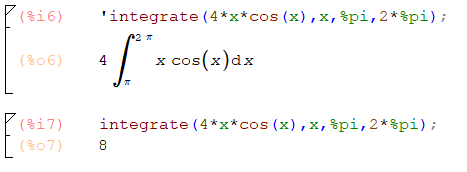
\includegraphics[width=0.4\linewidth]{def_ej.PNG}
\end{figure}

\subsection{Integral Numérica}

En caso de querer hacer una integral numérica, hay dos formas de hacer esto: una es mediante una función que hace específicamente la integral de forma numérica, mientras que la otra solo es con el comando "float" antes de el comando "integrate".

Primero vamos a ver el la integral numérica mediante el comando "quad\_qags". Éste hace uso de funciones cuadraticas para aproximar un valor altamente preciso. Este comando te presenta cuatro valores en forma de lista entre corchetes, donde el primer valor es la aproximación, la segunda el error máximo estimado, la tercera es información del número de funciones cuadraticas utilizadas para aproximar la curva y la última te da un código de ERROR. Los últimos dos no nos presenta información necesaria, por lo que podemos exigirle al comando que solo nos muestre el resultado de la siguiente manera:

\begin{center}
quad\_qags(f(x),x,a,b)[1]
\end{center}
donde
\begin{itemize}
\item f(x) es la función deseada a integrar.
\item x es con respecto a qué se va a integrar. 
\item a es el límite inferior de integración.
\item b es el límite superior de integración.
\item el "1" entre corchetes es para que solo se muestre el resultado de la integral aproximada. Se puede sustituir por un "2" para que muestre el error máximo estimado. En caso de querer mostrar la lista con los cuatro valores, se quita todo el corchete. 
\end{itemize}

\begin{figure}[h!]
  \centering
  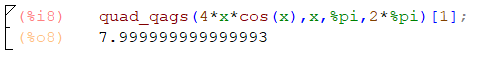
\includegraphics[width=0.4\linewidth]{numerico_ej.PNG}
\end{figure}

\subsection{Integrales Dobles}

Para hacer integrales dobles existen paquetes que te permiten hacerlo, pero los que se han encontrado han fallado, o no son muy eficientes al usarse; por lo que, personalmente, la forma más sencilla de hacerlo es con un comando "integrate", dentro de otro comando "integrate", de la siguiente manera:
\begin{center}
integrate(integrate(f(x,y),x,a,b),y,c,d)
\end{center}
donde
\begin{itemize}
\item f(x,y) es la función deseada a integrar.
\item x es con respecto a qué se va a integrar la primera vez. 
\item a es el límite inferior de integración, puede ser una función.
\item b es el límite superior de integración, puede ser una función.
\item y es con respecto a que se va a integrar la segunda vez.
\item c es el límite inferior de integración.
\item d es el límite superior de integración.
\end{itemize}

Éste mismo método puede ser aplicado para una integral triple.

\begin{figure}[h!]
  \centering
  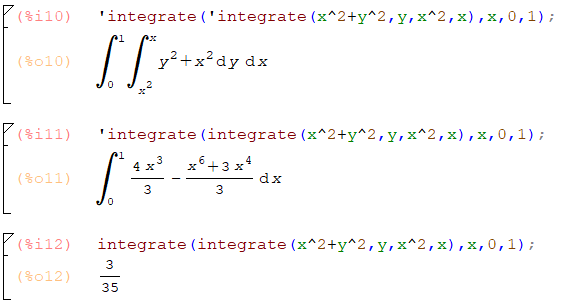
\includegraphics[width=0.6\linewidth]{dblint_ej.PNG}
\end{figure}

\subsection{Cambio de Variable}

Una herramienta importante para la integración es el cambio de variable. Maxima cuenta con un comando que te permite hacerlo:
\begin{center}
changevar(expresión,f(x,y),z,y)
\end{center}
donde
\begin{itemize}
\item expresión va el comando "integrate" con la integral que se desea hacer, ya sea definida o indefinida.
\item f(x,y) es la función con la que se va a cambiar la expresión; ésta está igualada a cero.
\item z es la nueva variable que va a aparecer en la función. 
\item y es la variable que se va a sustituir en la función.
\end{itemize}

\begin{figure}[h!]
  \centering
  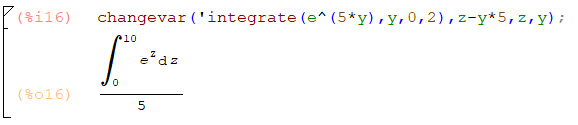
\includegraphics[width=0.6\linewidth]{changevar_ej.PNG}
\end{figure}

\section{Problema a Resolver}
A continuación, vamos a usar Maxima para resolver un problema de una tarea del curso de Calculo Integral y Diferencial IV. El problema dice así:

Calcule el volumen del sólido acotado por las dos superficies: $z = x^2 + 3y^2$ y $z = 4 - y^2$.

El valor calculado a mano fue $\frac{32}{3}$. Lo que Maxima calcula es:

\begin{figure}[h!]
  \centering
  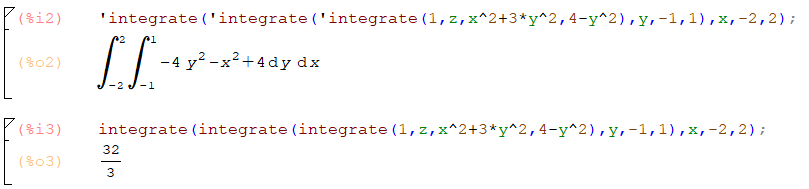
\includegraphics[width=0.8\linewidth]{Ej_1.PNG}
\end{figure}
\begin{figure}[h!]
  \centering
  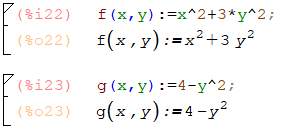
\includegraphics[width=0.2\linewidth]{Ej_2.PNG}
\end{figure}
\begin{figure}[h!]
  \centering
  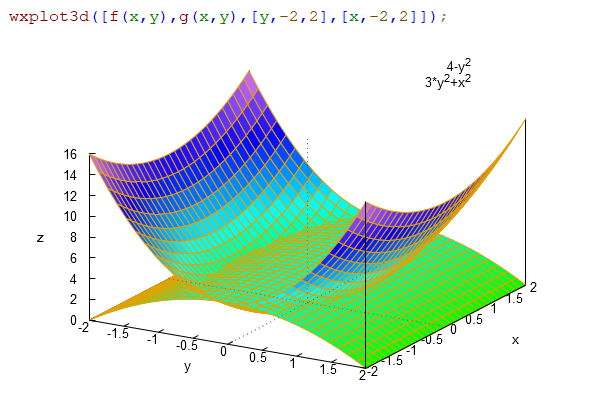
\includegraphics[width=0.8\linewidth]{Ej_3.PNG}
\end{figure}

Con esto, podemos confirmar que los resultados calculados a mano son correctos.

\section{Conclusión}
Explorar Maxima ha sido interesante, cuenta con muchas herramientas que pueden ser de mucho apoyo para muchos cursos de la carrera. La actividad ha sido completada sin ningún problema, ya que solo era leer los manuales, explorar un poco el software y crear uno en base a eso, no es algo muy complicado, además de que cumplió su objetivo de introducirnos a Maxima.


\section{Apéndice}
\begin{enumerate}
\item \textbf{¿Cuál fue tu primera impresión de wxmaxima?}
Es interesante conocer esta herramienta, ya que puede ser muy útil en el futuro. 
\item \textbf{¿Crees que esta herramienta puede ser útil en otros de tus cursos?}
Sí, con esta actividad acabo de notar que me puede ser muy útil con cálculo, hubiera sido de muy buena ayuda conocerla antes, pero no hay duda que más adelante algún provecho le podre sacar a este software. 
\item \textbf{¿Qué se te dificultó mas en esta actividad?}
Nada, los comandos y la infraestructura básica es muy fácil de explorar y entender.
\item \textbf{¿Se te hizo compleja esta actividad? ¿Cómo la mejorarías?}
No fue compleja y así como fue la actividad se me hizo muy bien. 
\end{enumerate}

\end{document}